\chapter{Container-Runtimes}
\label{chap:compCtnrRuntimes}

Container-Runtimes sind das Herz eines jeden Container-Angebots. Sie laden benötigte Images herunter und instanziieren übergebene Prozesse in Containern. In diesem Kapitel werden verschiedene Runtimes miteinander verglichen und veranschaulicht, wie Runtimes neben Docker für spezielle Anforderungen geeignet sind.

\section{Vorgehen}
\label{sec:vorgehen}
Um verschiedene Runtimes zu vergleichen wurde eine eigene Anwendung mit drei Microservices implementiert. Dabei wurden, wie in \fref{fig:todosStack} zu sehen, verschiedene Technologien verwendet, um zu prüfen, wie die getesteten Container-Runtimes mit diesen umgehen. Diese wurde im Folgenden mit verschiedenen Runtimes bereitgestellt.

\begin{figure}[h]
	\begin{center}
		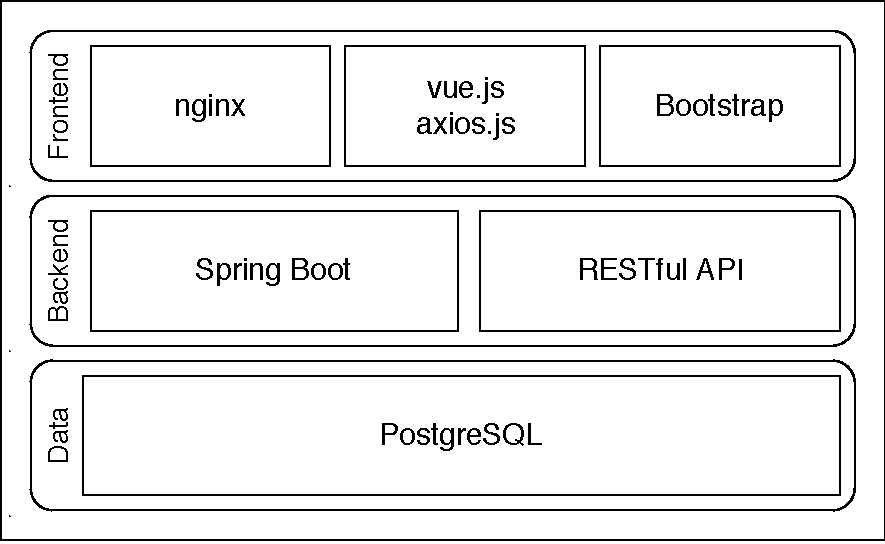
\includegraphics[width=0.8\textwidth]{bilder/microservice-example-stack.pdf}
		\caption{Beispielhafte Darstellung einer Micorservice-Architektur}
		\label{fig:todosStack}
	\end{center}
\end{figure}

Um verschiedene Runtimes objektiv zu bewerten wurden dabei die folgenden Kriterien untersucht.
\begin{itemize}
	\item Installations- und Konfigurationsaufwand
	\item Ease of Use
	\item Orchestrierung
	\item Sicherheit
	\item Aufnahme in bestehende Ecosysteme
\end{itemize}

Dabei wurde für jede Runtime dieselbe Ausgangssituation, eine virtuelle Maschine mit installiertem Ubuntu Xenial, gewählt.

\section{Docker Stack}
\label{sec:compDocker}
Docker ist de facto der Standard der Container-Runtimes. Dabei verwendet Docker als Runtime intern die unter der \gls{acr-cncf} veröffentlichte Runtime containerd, die wiederum ein Aufsatz zur standardisierten Runtime runC ist (Siehe \fref{fig:dockerStack}).

\begin{figure}[h]
	\begin{center}
		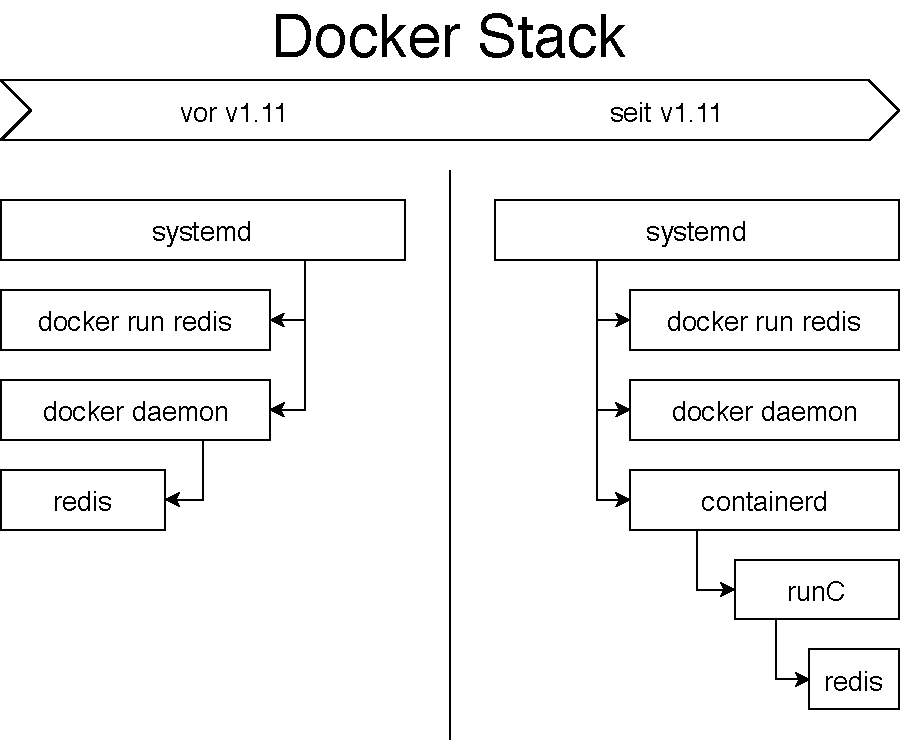
\includegraphics[width=\textwidth]{bilder/docker-stack-containerd-runc.pdf}
		\caption{Docker Stack im Laufe der Zeit \citep{RktVsOtherProjects}.}
		\label{fig:dockerStack}
	\end{center}
\end{figure}